% Options for packages loaded elsewhere
\PassOptionsToPackage{unicode}{hyperref}
\PassOptionsToPackage{hyphens}{url}
%
\documentclass[
]{article}
\usepackage{amsmath,amssymb}
\usepackage{lmodern}
\usepackage{iftex}
\ifPDFTeX
  \usepackage[T1]{fontenc}
  \usepackage[utf8]{inputenc}
  \usepackage{textcomp} % provide euro and other symbols
\else % if luatex or xetex
  \usepackage{unicode-math}
  \defaultfontfeatures{Scale=MatchLowercase}
  \defaultfontfeatures[\rmfamily]{Ligatures=TeX,Scale=1}
\fi
% Use upquote if available, for straight quotes in verbatim environments
\IfFileExists{upquote.sty}{\usepackage{upquote}}{}
\IfFileExists{microtype.sty}{% use microtype if available
  \usepackage[]{microtype}
  \UseMicrotypeSet[protrusion]{basicmath} % disable protrusion for tt fonts
}{}
\makeatletter
\@ifundefined{KOMAClassName}{% if non-KOMA class
  \IfFileExists{parskip.sty}{%
    \usepackage{parskip}
  }{% else
    \setlength{\parindent}{0pt}
    \setlength{\parskip}{6pt plus 2pt minus 1pt}}
}{% if KOMA class
  \KOMAoptions{parskip=half}}
\makeatother
\usepackage{xcolor}
\usepackage[margin=1in]{geometry}
\usepackage{color}
\usepackage{fancyvrb}
\newcommand{\VerbBar}{|}
\newcommand{\VERB}{\Verb[commandchars=\\\{\}]}
\DefineVerbatimEnvironment{Highlighting}{Verbatim}{commandchars=\\\{\}}
% Add ',fontsize=\small' for more characters per line
\usepackage{framed}
\definecolor{shadecolor}{RGB}{248,248,248}
\newenvironment{Shaded}{\begin{snugshade}}{\end{snugshade}}
\newcommand{\AlertTok}[1]{\textcolor[rgb]{0.94,0.16,0.16}{#1}}
\newcommand{\AnnotationTok}[1]{\textcolor[rgb]{0.56,0.35,0.01}{\textbf{\textit{#1}}}}
\newcommand{\AttributeTok}[1]{\textcolor[rgb]{0.77,0.63,0.00}{#1}}
\newcommand{\BaseNTok}[1]{\textcolor[rgb]{0.00,0.00,0.81}{#1}}
\newcommand{\BuiltInTok}[1]{#1}
\newcommand{\CharTok}[1]{\textcolor[rgb]{0.31,0.60,0.02}{#1}}
\newcommand{\CommentTok}[1]{\textcolor[rgb]{0.56,0.35,0.01}{\textit{#1}}}
\newcommand{\CommentVarTok}[1]{\textcolor[rgb]{0.56,0.35,0.01}{\textbf{\textit{#1}}}}
\newcommand{\ConstantTok}[1]{\textcolor[rgb]{0.00,0.00,0.00}{#1}}
\newcommand{\ControlFlowTok}[1]{\textcolor[rgb]{0.13,0.29,0.53}{\textbf{#1}}}
\newcommand{\DataTypeTok}[1]{\textcolor[rgb]{0.13,0.29,0.53}{#1}}
\newcommand{\DecValTok}[1]{\textcolor[rgb]{0.00,0.00,0.81}{#1}}
\newcommand{\DocumentationTok}[1]{\textcolor[rgb]{0.56,0.35,0.01}{\textbf{\textit{#1}}}}
\newcommand{\ErrorTok}[1]{\textcolor[rgb]{0.64,0.00,0.00}{\textbf{#1}}}
\newcommand{\ExtensionTok}[1]{#1}
\newcommand{\FloatTok}[1]{\textcolor[rgb]{0.00,0.00,0.81}{#1}}
\newcommand{\FunctionTok}[1]{\textcolor[rgb]{0.00,0.00,0.00}{#1}}
\newcommand{\ImportTok}[1]{#1}
\newcommand{\InformationTok}[1]{\textcolor[rgb]{0.56,0.35,0.01}{\textbf{\textit{#1}}}}
\newcommand{\KeywordTok}[1]{\textcolor[rgb]{0.13,0.29,0.53}{\textbf{#1}}}
\newcommand{\NormalTok}[1]{#1}
\newcommand{\OperatorTok}[1]{\textcolor[rgb]{0.81,0.36,0.00}{\textbf{#1}}}
\newcommand{\OtherTok}[1]{\textcolor[rgb]{0.56,0.35,0.01}{#1}}
\newcommand{\PreprocessorTok}[1]{\textcolor[rgb]{0.56,0.35,0.01}{\textit{#1}}}
\newcommand{\RegionMarkerTok}[1]{#1}
\newcommand{\SpecialCharTok}[1]{\textcolor[rgb]{0.00,0.00,0.00}{#1}}
\newcommand{\SpecialStringTok}[1]{\textcolor[rgb]{0.31,0.60,0.02}{#1}}
\newcommand{\StringTok}[1]{\textcolor[rgb]{0.31,0.60,0.02}{#1}}
\newcommand{\VariableTok}[1]{\textcolor[rgb]{0.00,0.00,0.00}{#1}}
\newcommand{\VerbatimStringTok}[1]{\textcolor[rgb]{0.31,0.60,0.02}{#1}}
\newcommand{\WarningTok}[1]{\textcolor[rgb]{0.56,0.35,0.01}{\textbf{\textit{#1}}}}
\usepackage{graphicx}
\makeatletter
\def\maxwidth{\ifdim\Gin@nat@width>\linewidth\linewidth\else\Gin@nat@width\fi}
\def\maxheight{\ifdim\Gin@nat@height>\textheight\textheight\else\Gin@nat@height\fi}
\makeatother
% Scale images if necessary, so that they will not overflow the page
% margins by default, and it is still possible to overwrite the defaults
% using explicit options in \includegraphics[width, height, ...]{}
\setkeys{Gin}{width=\maxwidth,height=\maxheight,keepaspectratio}
% Set default figure placement to htbp
\makeatletter
\def\fps@figure{htbp}
\makeatother
\setlength{\emergencystretch}{3em} % prevent overfull lines
\providecommand{\tightlist}{%
  \setlength{\itemsep}{0pt}\setlength{\parskip}{0pt}}
\setcounter{secnumdepth}{-\maxdimen} % remove section numbering
\ifLuaTeX
  \usepackage{selnolig}  % disable illegal ligatures
\fi
\IfFileExists{bookmark.sty}{\usepackage{bookmark}}{\usepackage{hyperref}}
\IfFileExists{xurl.sty}{\usepackage{xurl}}{} % add URL line breaks if available
\urlstyle{same} % disable monospaced font for URLs
\hypersetup{
  pdftitle={hw02},
  pdfauthor={Samuel Swain},
  hidelinks,
  pdfcreator={LaTeX via pandoc}}

\title{hw02}
\author{Samuel Swain}
\date{2023-02-10}

\begin{document}
\maketitle

\begin{verbatim}
## Loading required package: Matrix
\end{verbatim}

\begin{verbatim}
## Loaded glmnet 4.1-4
\end{verbatim}

\hypertarget{problem-1}{%
\section{Problem 1}\label{problem-1}}

\hypertarget{a}{%
\subsubsection{1(a)}\label{a}}

\begin{verbatim}
## MSE: 
##  - Average: 1.947016 
##  - SD 0.02844145
\end{verbatim}

As we can see above, the average error is 1.9470162 per prediction with
a standard deviation of 0.0284414. The predictive power of this model
can definitely be improved or we can explore other models that will do a
better job at predicting cost.

\hypertarget{b}{%
\subsubsection{1(b)}\label{b}}

\begin{verbatim}
## 
## Call:
## lm(formula = cost ~ age + gend + intvn + drugs + ervis, data = df_1)
## 
## Residuals:
##     Min      1Q  Median      3Q     Max 
## -7.0979 -0.7699  0.1101  0.8554  3.3293 
## 
## Coefficients:
##              Estimate Std. Error t value Pr(>|t|)    
## (Intercept)  6.290013   0.048606 129.408  < 2e-16 ***
## age          0.001477   0.048832   0.030  0.97587    
## gend        -0.071141   0.048982  -1.452  0.14680    
## intvn        1.283944   0.052426  24.491  < 2e-16 ***
## drugs       -0.088402   0.057351  -1.541  0.12362    
## ervis        0.178760   0.060489   2.955  0.00322 ** 
## ---
## Signif. codes:  0 '***' 0.001 '**' 0.01 '*' 0.05 '.' 0.1 ' ' 1
## 
## Residual standard error: 1.364 on 782 degrees of freedom
## Multiple R-squared:  0.491,  Adjusted R-squared:  0.4877 
## F-statistic: 150.9 on 5 and 782 DF,  p-value: < 2.2e-16
\end{verbatim}

Total number of interventions and number emergency room visits seem to
have the highest effect on the cost of the subscriber. Increasing intvn
by only one will increase the cost of the subscriber by about 812.08
whereas increasing ervis by just one will also increase the cost of the
subscriber by about 376.53 dollars.

\hypertarget{c}{%
\subsubsection{1(c)}\label{c}}

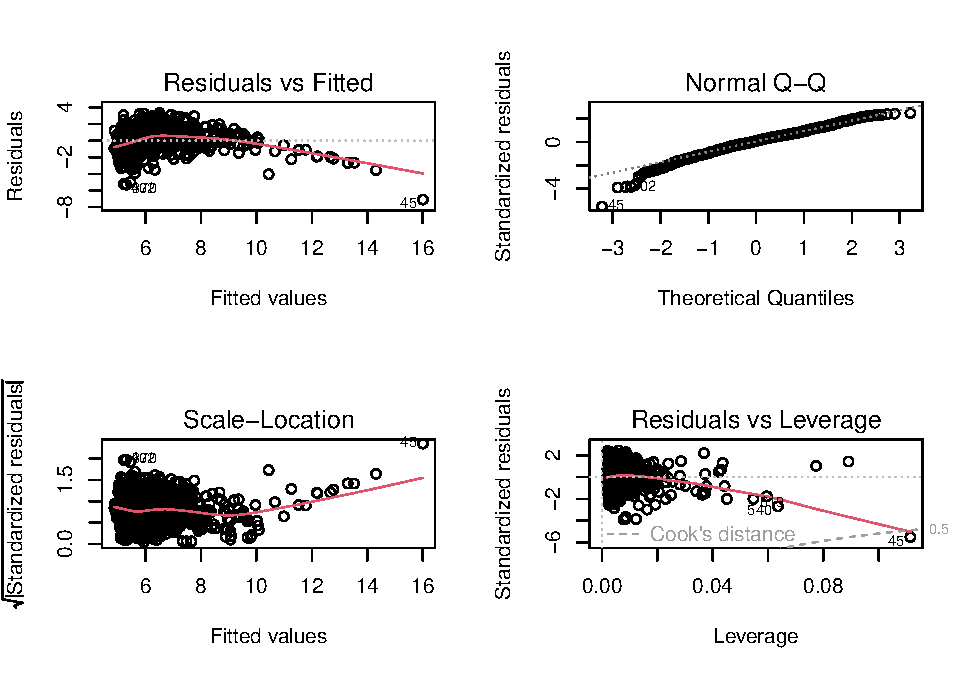
\includegraphics{hw02_files/figure-latex/question_1c-1.pdf}

As we can see from the plots above, there are a lot of problems with
using a linear model to attain the relationship between the features and
the cost. The problems are listed below: - Non-linearity of the data
based on the Residuals vs Fitted plot - A few outliers based on the
Residuals vs Leverage plot

\hypertarget{problem-2}{%
\section{Problem 2}\label{problem-2}}

\hypertarget{a-1}{%
\subsubsection{2(a)}\label{a-1}}

\begin{verbatim}
## Best NNet: 
##  Model: 1 
##  Decay: 15 
##  Size: 0.5
\end{verbatim}

\hypertarget{b-1}{%
\subsubsection{2(b)}\label{b-1}}

\begin{verbatim}
## MSE: 
##  - Average: 1.458738 
##  - SD 0.04090414
\end{verbatim}

The best Neural Net attained above has a size of 15 and a decay rate of
0.5. In terms of predictive power, I think the model is very good. With
an average CV MSE of 1.9754511, it performs better than the linear
model.

\hypertarget{c-1}{%
\subsubsection{2(c)}\label{c-1}}

\includegraphics{hw02_files/figure-latex/question_2c-1.pdf}

Below are the top three features ranked by strength of effect: -
Intervention (intvn): Positive - Complications (comp): Positive for the
first 25\% and then negative for the last 75\% - Drugs (drugs): Negative
for the first 20\% and then negative for the last 80\%

\hypertarget{d}{%
\subsubsection{2(d)}\label{d}}

\includegraphics{hw02_files/figure-latex/question_2d-1.pdf}

Looking at the fitted versus residual plot above, we can see pretty much
all of the non linearity has been captured.

\hypertarget{problem-3}{%
\section{Problem 3}\label{problem-3}}

\hypertarget{a-2}{%
\subsubsection{3(a)}\label{a-2}}

\begin{verbatim}
## Best Tree: 
##  Model: 2 
##  Minbucket: 10 
##  CP: 0.001
\end{verbatim}

\hypertarget{b-2}{%
\subsubsection{3(b)}\label{b-2}}

\begin{verbatim}
## MSE: 
##  - Average: 1.281127 
##  - SD 0.0268458
\end{verbatim}

The best Tree attained above has a min-bucket of 10 and a decay rate of
0.001. In terms of predictive power, I think the model is really good.
It's better at predicting than the linear and N Net model given average
CV MSE of 1.2811271.

\hypertarget{c-2}{%
\subsubsection{3(c)}\label{c-2}}

\includegraphics{hw02_files/figure-latex/question_3c-1.pdf}

As we can see above, intervention (intvn) is again the most important
variable when fitting the tree. The cost of the subscriber goes up for
each additional intervention until two, then the effect levels off.
Another important variable is comorb. We can see that the effect is not
as big as intvn but it still explains about 1.5 total variation in cost.

\hypertarget{d-1}{%
\subsubsection{3(d)}\label{d-1}}

\includegraphics{hw02_files/figure-latex/question_3d-1.pdf}

The pattern of this tree Fitted vs Residual plot is similar to the N Net
plot. It seems to have captured most of the non linearity. There is no
trend down or up as we increase fitted values.

\hypertarget{e}{%
\subsubsection{3(e)}\label{e}}

I would use the tree model as it produces the lowest MSE out of the
three models. It also is able to capture all of the non linearity in the
data.

\hypertarget{question-4}{%
\section{Question 4}\label{question-4}}

\hypertarget{a-3}{%
\subsubsection{4(a)}\label{a-3}}

\begin{verbatim}
## Best NNet: 
##  Model: 2 
##  Size: 20 
##  Decay: 0.1
\end{verbatim}

\hypertarget{b-3}{%
\subsubsection{4(b)}\label{b-3}}

\begin{verbatim}
## Best Tree: 
##  Model: 2 
##  CP: 1e-04 
##  Minbucket: 5
\end{verbatim}

\hypertarget{c-3}{%
\subsubsection{4(c)}\label{c-3}}

\hypertarget{d-2}{%
\subsubsection{4(d)}\label{d-2}}

\begin{verbatim}
## Models 
##  - NNet: 0.6137072 
##  - Tree: 0.7009346 
##  - MNLogit: 0.5934579
\end{verbatim}

The logit model is more interpretable than the nnet but about the same
as the tree model. The only extra piece of information the logit model
gives us is access to the exact change in likelihoods / probabilities
from looking at the coefficients. The tree model has a higher cross
validation accuracy as well as similar interpretability. We should
choose the tree model over the nnet all day. When looking at the MNlogit
model we see that it gets about 0.0872274 less predictions correct.
Given the slightly higher interpretability of the MNlogit model versus
the much higher prediction accuracy of the Tree model, using the Tree
model will be more appropriate for predicting glass type.

\hypertarget{appendix}{%
\section{Appendix}\label{appendix}}

\hypertarget{commented-out-code-is-the-output-used-to-attain-the-results-above.-commended-to-shorted-final-submission-pdf.}{%
\subsubsection{Commented out code is the output used to attain the
results above. Commended to shorted final submission
pdf.}\label{commented-out-code-is-the-output-used-to-attain-the-results-above.-commended-to-shorted-final-submission-pdf.}}

\begin{Shaded}
\begin{Highlighting}[]
\CommentTok{\# Libraries}
\FunctionTok{library}\NormalTok{(boot)}
\FunctionTok{library}\NormalTok{(nnet)}
\FunctionTok{library}\NormalTok{(glmnet)}
\FunctionTok{library}\NormalTok{(ALEPlot)}
\FunctionTok{library}\NormalTok{(rpart)}

\CommentTok{\# Cross Validation}
\NormalTok{CVInd }\OtherTok{\textless{}{-}} \ControlFlowTok{function}\NormalTok{(n,K) \{ }
  \CommentTok{\# n is sample size; K is number of parts; }
  \CommentTok{\# returns K{-}length list of indices for each part}
\NormalTok{  m}\OtherTok{\textless{}{-}}\FunctionTok{floor}\NormalTok{(n}\SpecialCharTok{/}\NormalTok{K) }\CommentTok{\#approximate size of each part}
\NormalTok{  r}\OtherTok{\textless{}{-}}\NormalTok{n}\SpecialCharTok{{-}}\NormalTok{m}\SpecialCharTok{*}\NormalTok{K}
\NormalTok{  I}\OtherTok{\textless{}{-}}\FunctionTok{sample}\NormalTok{(n,n) }\CommentTok{\#random reordering of the indices}
\NormalTok{  Ind}\OtherTok{\textless{}{-}}\FunctionTok{list}\NormalTok{() }\CommentTok{\#will be list of indices for all K parts}
  \FunctionTok{length}\NormalTok{(Ind)}\OtherTok{\textless{}{-}}\NormalTok{K}
  \ControlFlowTok{for}\NormalTok{ (k }\ControlFlowTok{in} \DecValTok{1}\SpecialCharTok{:}\NormalTok{K) \{}
    \ControlFlowTok{if}\NormalTok{ (k }\SpecialCharTok{\textless{}=}\NormalTok{ r) kpart }\OtherTok{\textless{}{-}}\NormalTok{ ((m}\SpecialCharTok{+}\DecValTok{1}\NormalTok{)}\SpecialCharTok{*}\NormalTok{(k}\DecValTok{{-}1}\NormalTok{)}\SpecialCharTok{+}\DecValTok{1}\NormalTok{)}\SpecialCharTok{:}\NormalTok{((m}\SpecialCharTok{+}\DecValTok{1}\NormalTok{)}\SpecialCharTok{*}\NormalTok{k)}
    \ControlFlowTok{else}\NormalTok{ kpart}\OtherTok{\textless{}{-}}\NormalTok{((m}\SpecialCharTok{+}\DecValTok{1}\NormalTok{)}\SpecialCharTok{*}\NormalTok{r}\SpecialCharTok{+}\NormalTok{m}\SpecialCharTok{*}\NormalTok{(k}\SpecialCharTok{{-}}\NormalTok{r}\DecValTok{{-}1}\NormalTok{)}\SpecialCharTok{+}\DecValTok{1}\NormalTok{)}\SpecialCharTok{:}\NormalTok{((m}\SpecialCharTok{+}\DecValTok{1}\NormalTok{)}\SpecialCharTok{*}\NormalTok{r}\SpecialCharTok{+}\NormalTok{m}\SpecialCharTok{*}\NormalTok{(k}\SpecialCharTok{{-}}\NormalTok{r))}
\NormalTok{    Ind[[k]] }\OtherTok{\textless{}{-}}\NormalTok{ I[kpart] }\CommentTok{\#indices for kth part of data}
\NormalTok{  \}}
\NormalTok{  Ind}
\NormalTok{\}}

\CommentTok{\# Standardize Function}
\NormalTok{standardize\_predictors }\OtherTok{\textless{}{-}} \ControlFlowTok{function}\NormalTok{(data) \{}
\NormalTok{  predictors }\OtherTok{\textless{}{-}}\NormalTok{ data}
\NormalTok{  standardized\_predictors }\OtherTok{\textless{}{-}} \FunctionTok{scale}\NormalTok{(predictors)}
\NormalTok{  data }\OtherTok{\textless{}{-}}\NormalTok{ standardized\_predictors}
  \FunctionTok{return}\NormalTok{(data)}
\NormalTok{\}}
\end{Highlighting}
\end{Shaded}

\hypertarget{problem-1-1}{%
\section{Problem 1}\label{problem-1-1}}

\begin{Shaded}
\begin{Highlighting}[]
\FunctionTok{library}\NormalTok{(readxl)}
\NormalTok{df\_1 }\OtherTok{=} \FunctionTok{read\_excel}\NormalTok{(}\StringTok{"HW2\_data.xls"}\NormalTok{)}
\NormalTok{df\_1 }\OtherTok{=}\NormalTok{ df\_1[, }\SpecialCharTok{{-}}\FunctionTok{c}\NormalTok{(}\DecValTok{1}\NormalTok{)]}

\CommentTok{\# Vars}
\NormalTok{df\_1}\SpecialCharTok{$}\NormalTok{cost}\OtherTok{\textless{}{-}}\FunctionTok{log}\NormalTok{(df\_1}\SpecialCharTok{$}\NormalTok{cost)}
\NormalTok{X\_1 }\OtherTok{=}\NormalTok{ df\_1[, }\SpecialCharTok{{-}}\FunctionTok{c}\NormalTok{(}\DecValTok{1}\NormalTok{)]}
\NormalTok{df\_1[, }\FunctionTok{c}\NormalTok{(}\DecValTok{2}\NormalTok{, }\DecValTok{3}\NormalTok{, }\DecValTok{4}\NormalTok{, }\DecValTok{5}\NormalTok{, }\DecValTok{6}\NormalTok{, }\DecValTok{7}\NormalTok{, }\DecValTok{8}\NormalTok{, }\DecValTok{9}\NormalTok{)] }\OtherTok{=} \FunctionTok{standardize\_predictors}\NormalTok{(X\_1)}
\end{Highlighting}
\end{Shaded}

\hypertarget{a-4}{%
\subsubsection{1(a)}\label{a-4}}

code:

\begin{Shaded}
\begin{Highlighting}[]
\NormalTok{fit\_1a }\OtherTok{\textless{}{-}} \FunctionTok{lm}\NormalTok{(cost }\SpecialCharTok{\textasciitilde{}}\NormalTok{ age }\SpecialCharTok{+}\NormalTok{ gend }\SpecialCharTok{+}\NormalTok{ intvn }\SpecialCharTok{+}\NormalTok{ drugs }\SpecialCharTok{+}\NormalTok{ ervis, }\AttributeTok{data =}\NormalTok{ df\_1)}

\DocumentationTok{\#\#Now use multiple reps of CV to compare Neural Nets and linear reg models\#\#\#}
\NormalTok{Nrep}\OtherTok{\textless{}{-}}\DecValTok{5} \CommentTok{\#number of replicates of CV}
\NormalTok{K}\OtherTok{\textless{}{-}}\DecValTok{3}  \CommentTok{\#K{-}fold CV on each replicate}
\NormalTok{n.models }\OtherTok{=} \DecValTok{1} \CommentTok{\#number of different models to fit}
\NormalTok{n}\OtherTok{=}\FunctionTok{nrow}\NormalTok{(df\_1)}
\NormalTok{y}\OtherTok{\textless{}{-}}\NormalTok{df\_1}\SpecialCharTok{$}\NormalTok{cost}
\NormalTok{yhat}\OtherTok{=}\FunctionTok{matrix}\NormalTok{(}\DecValTok{0}\NormalTok{,n,n.models)}
\NormalTok{MSE}\OtherTok{\textless{}{-}}\FunctionTok{matrix}\NormalTok{(}\DecValTok{0}\NormalTok{,Nrep,n.models)}
\NormalTok{RMSE}\OtherTok{\textless{}{-}}\FunctionTok{matrix}\NormalTok{(}\DecValTok{0}\NormalTok{,Nrep,n.models)}
\ControlFlowTok{for}\NormalTok{ (j }\ControlFlowTok{in} \DecValTok{1}\SpecialCharTok{:}\NormalTok{Nrep) \{}
\NormalTok{  Ind}\OtherTok{\textless{}{-}}\FunctionTok{CVInd}\NormalTok{(n,K)}
  \ControlFlowTok{for}\NormalTok{ (k }\ControlFlowTok{in} \DecValTok{1}\SpecialCharTok{:}\NormalTok{K) \{}
\NormalTok{    out}\OtherTok{\textless{}{-}}\FunctionTok{lm}\NormalTok{(cost }\SpecialCharTok{\textasciitilde{}}\NormalTok{ age }\SpecialCharTok{+}\NormalTok{ gend }\SpecialCharTok{+}\NormalTok{ intvn }\SpecialCharTok{+}\NormalTok{ drugs }\SpecialCharTok{+}\NormalTok{ ervis, }\AttributeTok{data =}\NormalTok{ df\_1[}\SpecialCharTok{{-}}\NormalTok{Ind[[k]],])}
\NormalTok{    yhat[Ind[[k]],}\DecValTok{1}\NormalTok{]}\OtherTok{\textless{}{-}}\FunctionTok{as.numeric}\NormalTok{(}\FunctionTok{predict}\NormalTok{(out,df\_1[Ind[[k]],]))}
\NormalTok{  \} }\CommentTok{\#end of k loop}
\NormalTok{  MSE[j,]}\OtherTok{=}\FunctionTok{apply}\NormalTok{(yhat,}\DecValTok{2}\NormalTok{,}\ControlFlowTok{function}\NormalTok{(x) }\FunctionTok{sum}\NormalTok{((y}\SpecialCharTok{{-}}\NormalTok{x)}\SpecialCharTok{\^{}}\DecValTok{2}\NormalTok{))}\SpecialCharTok{/}\NormalTok{n}
\NormalTok{  RMSE[j,]}\OtherTok{=}\FunctionTok{apply}\NormalTok{(yhat,}\DecValTok{2}\NormalTok{,}\ControlFlowTok{function}\NormalTok{(x) }\FunctionTok{sqrt}\NormalTok{(}\FunctionTok{sum}\NormalTok{((y}\SpecialCharTok{{-}}\NormalTok{x)}\SpecialCharTok{\^{}}\DecValTok{2}\NormalTok{))}\SpecialCharTok{/}\NormalTok{n)}
\NormalTok{\} }\CommentTok{\#end of j loop}
\NormalTok{MSEAve}\OtherTok{\textless{}{-}} \FunctionTok{apply}\NormalTok{(MSE,}\DecValTok{2}\NormalTok{,mean) }\CommentTok{\#averaged mean square CV error}
\NormalTok{MSEsd }\OtherTok{\textless{}{-}} \FunctionTok{apply}\NormalTok{(MSE,}\DecValTok{2}\NormalTok{,sd)   }\CommentTok{\#SD of mean square CV error}
\NormalTok{RMSEAve}\OtherTok{\textless{}{-}} \FunctionTok{apply}\NormalTok{(RMSE,}\DecValTok{2}\NormalTok{,mean) }\CommentTok{\#averaged mean square CV error}
\NormalTok{RMSEsd }\OtherTok{\textless{}{-}} \FunctionTok{apply}\NormalTok{(RMSE,}\DecValTok{2}\NormalTok{,sd)   }\CommentTok{\#SD of mean square CV error}

\CommentTok{\# cat("MSE:", "\textbackslash{}n", "{-} Average:", MSEAve, "\textbackslash{}n", "{-} SD", MSEsd)}
\end{Highlighting}
\end{Shaded}

\hypertarget{b-4}{%
\subsubsection{1(b)}\label{b-4}}

code:

\begin{Shaded}
\begin{Highlighting}[]
\CommentTok{\# summary(fit\_1a)}
\end{Highlighting}
\end{Shaded}

\hypertarget{c-4}{%
\subsubsection{1(c)}\label{c-4}}

code:

\begin{Shaded}
\begin{Highlighting}[]
\CommentTok{\# par(mfrow = c(2,2))}
\CommentTok{\# plot(fit\_1a)}
\end{Highlighting}
\end{Shaded}

\hypertarget{problem-2-1}{%
\section{Problem 2}\label{problem-2-1}}

\hypertarget{a-5}{%
\subsubsection{2(a)}\label{a-5}}

code:

\begin{Shaded}
\begin{Highlighting}[]
\DocumentationTok{\#\#Now use multiple reps of CV to compare Neural Nets and linear reg models\#\#\#}
\NormalTok{Nrep}\OtherTok{\textless{}{-}}\DecValTok{3} \CommentTok{\#number of replicates of CV}
\NormalTok{K}\OtherTok{\textless{}{-}}\DecValTok{10}  \CommentTok{\#K{-}fold CV on each replicate}
\NormalTok{n.models }\OtherTok{=} \DecValTok{4} \CommentTok{\#number of different models to fit}
\NormalTok{n}\OtherTok{=}\FunctionTok{nrow}\NormalTok{(df\_1)}
\NormalTok{y}\OtherTok{\textless{}{-}}\NormalTok{df\_1}\SpecialCharTok{$}\NormalTok{cost}
\NormalTok{yhat}\OtherTok{=}\FunctionTok{matrix}\NormalTok{(}\DecValTok{0}\NormalTok{,n,n.models)}
\NormalTok{MSE}\OtherTok{\textless{}{-}}\FunctionTok{matrix}\NormalTok{(}\DecValTok{0}\NormalTok{,Nrep,n.models)}
\ControlFlowTok{for}\NormalTok{ (j }\ControlFlowTok{in} \DecValTok{1}\SpecialCharTok{:}\NormalTok{Nrep) \{}
\NormalTok{  Ind}\OtherTok{\textless{}{-}}\FunctionTok{CVInd}\NormalTok{(n,K)}
  \ControlFlowTok{for}\NormalTok{ (k }\ControlFlowTok{in} \DecValTok{1}\SpecialCharTok{:}\NormalTok{K) \{}
\NormalTok{    out}\OtherTok{\textless{}{-}}\FunctionTok{nnet}\NormalTok{(cost}\SpecialCharTok{\textasciitilde{}}\NormalTok{.,df\_1[}\SpecialCharTok{{-}}\NormalTok{Ind[[k]],], }\AttributeTok{linout=}\NormalTok{T, }\AttributeTok{skip=}\NormalTok{F, }\AttributeTok{size=}\DecValTok{15}\NormalTok{, }\AttributeTok{decay=}\NormalTok{.}\DecValTok{5}\NormalTok{, }\AttributeTok{maxit=}\DecValTok{1000}\NormalTok{, }\AttributeTok{trace=}\NormalTok{F)}
\NormalTok{    yhat[Ind[[k]],}\DecValTok{1}\NormalTok{]}\OtherTok{\textless{}{-}}\FunctionTok{as.numeric}\NormalTok{(}\FunctionTok{predict}\NormalTok{(out,df\_1[Ind[[k]],]))}
\NormalTok{    out}\OtherTok{\textless{}{-}}\FunctionTok{nnet}\NormalTok{(cost}\SpecialCharTok{\textasciitilde{}}\NormalTok{.,df\_1[}\SpecialCharTok{{-}}\NormalTok{Ind[[k]],], }\AttributeTok{linout=}\NormalTok{T, }\AttributeTok{skip=}\NormalTok{F, }\AttributeTok{size=}\DecValTok{20}\NormalTok{, }\AttributeTok{decay=}\NormalTok{.}\DecValTok{1}\NormalTok{, }\AttributeTok{maxit=}\DecValTok{1000}\NormalTok{, }\AttributeTok{trace=}\NormalTok{F)}
\NormalTok{    yhat[Ind[[k]],}\DecValTok{2}\NormalTok{]}\OtherTok{\textless{}{-}}\FunctionTok{as.numeric}\NormalTok{(}\FunctionTok{predict}\NormalTok{(out,df\_1[Ind[[k]],]))}
\NormalTok{    out}\OtherTok{\textless{}{-}}\FunctionTok{nnet}\NormalTok{(cost}\SpecialCharTok{\textasciitilde{}}\NormalTok{.,df\_1[}\SpecialCharTok{{-}}\NormalTok{Ind[[k]],], }\AttributeTok{linout=}\NormalTok{T, }\AttributeTok{skip=}\NormalTok{F, }\AttributeTok{size=}\DecValTok{25}\NormalTok{, }\AttributeTok{decay=}\NormalTok{.}\DecValTok{01}\NormalTok{, }\AttributeTok{maxit=}\DecValTok{1000}\NormalTok{, }\AttributeTok{trace=}\NormalTok{F)}
\NormalTok{    yhat[Ind[[k]],}\DecValTok{3}\NormalTok{]}\OtherTok{\textless{}{-}}\FunctionTok{as.numeric}\NormalTok{(}\FunctionTok{predict}\NormalTok{(out,df\_1[Ind[[k]],]))}
\NormalTok{    out}\OtherTok{\textless{}{-}}\FunctionTok{nnet}\NormalTok{(cost}\SpecialCharTok{\textasciitilde{}}\NormalTok{.,df\_1[}\SpecialCharTok{{-}}\NormalTok{Ind[[k]],], }\AttributeTok{linout=}\NormalTok{T, }\AttributeTok{skip=}\NormalTok{F, }\AttributeTok{size=}\DecValTok{30}\NormalTok{, }\AttributeTok{decay=}\DecValTok{0}\NormalTok{, }\AttributeTok{maxit=}\DecValTok{1000}\NormalTok{, }\AttributeTok{trace=}\NormalTok{F)}
\NormalTok{    yhat[Ind[[k]],}\DecValTok{4}\NormalTok{]}\OtherTok{\textless{}{-}}\FunctionTok{as.numeric}\NormalTok{(}\FunctionTok{predict}\NormalTok{(out,df\_1[Ind[[k]],]))}
\NormalTok{  \} }\CommentTok{\#end of k loop}
\NormalTok{  MSE[j,]}\OtherTok{=}\FunctionTok{apply}\NormalTok{(yhat,}\DecValTok{2}\NormalTok{,}\ControlFlowTok{function}\NormalTok{(x) }\FunctionTok{sum}\NormalTok{((y}\SpecialCharTok{{-}}\NormalTok{x)}\SpecialCharTok{\^{}}\DecValTok{2}\NormalTok{))}\SpecialCharTok{/}\NormalTok{n}
\NormalTok{\} }\CommentTok{\#end of j loop}
\CommentTok{\# MSE}
\NormalTok{MSEAve}\OtherTok{\textless{}{-}} \FunctionTok{apply}\NormalTok{(MSE,}\DecValTok{2}\NormalTok{,mean) }\CommentTok{\#averaged mean square CV error}
\NormalTok{MSEsd }\OtherTok{\textless{}{-}} \FunctionTok{apply}\NormalTok{(MSE,}\DecValTok{2}\NormalTok{,sd)  }\CommentTok{\#SD of mean square CV error}

\FunctionTok{cat}\NormalTok{(}\StringTok{"Best NNet:"}\NormalTok{, }\StringTok{"}\SpecialCharTok{\textbackslash{}n}\StringTok{"}\NormalTok{, }\StringTok{"Model:"}\NormalTok{, }\FunctionTok{which.min}\NormalTok{(MSEAve), }\StringTok{"}\SpecialCharTok{\textbackslash{}n}\StringTok{"}\NormalTok{, }
    \StringTok{"Decay:"}\NormalTok{, }\FunctionTok{c}\NormalTok{(}\DecValTok{15}\NormalTok{, }\DecValTok{20}\NormalTok{, }\DecValTok{25}\NormalTok{, }\DecValTok{30}\NormalTok{)[}\FunctionTok{which.min}\NormalTok{(MSEAve)], }\StringTok{"}\SpecialCharTok{\textbackslash{}n}\StringTok{"}\NormalTok{, }
    \StringTok{"Size:"}\NormalTok{, }\FunctionTok{c}\NormalTok{(}\FloatTok{0.5}\NormalTok{, }\FloatTok{0.1}\NormalTok{, }\FloatTok{0.01}\NormalTok{, }\DecValTok{0}\NormalTok{)[}\FunctionTok{which.min}\NormalTok{(MSEAve)])}
\end{Highlighting}
\end{Shaded}

\begin{verbatim}
## Best NNet: 
##  Model: 1 
##  Decay: 15 
##  Size: 0.5
\end{verbatim}

\hypertarget{b-5}{%
\subsubsection{2(b)}\label{b-5}}

code:

\begin{Shaded}
\begin{Highlighting}[]
\NormalTok{best\_nnet\_2b }\OtherTok{\textless{}{-}} \FunctionTok{nnet}\NormalTok{(cost}\SpecialCharTok{\textasciitilde{}}\NormalTok{., df\_1, }\AttributeTok{linout=}\NormalTok{T, }\AttributeTok{skip=}\NormalTok{F, }
                     \AttributeTok{size=}\FunctionTok{c}\NormalTok{(}\DecValTok{15}\NormalTok{, }\DecValTok{20}\NormalTok{, }\DecValTok{25}\NormalTok{, }\DecValTok{30}\NormalTok{)[}\FunctionTok{which.min}\NormalTok{(MSEAve)], }
                     \AttributeTok{decay=}\FunctionTok{c}\NormalTok{(}\FloatTok{0.5}\NormalTok{, }\FloatTok{0.1}\NormalTok{, }\FloatTok{0.01}\NormalTok{, }\DecValTok{0}\NormalTok{)[}\FunctionTok{which.min}\NormalTok{(MSEAve)], }
                     \AttributeTok{maxit=}\DecValTok{1000}\NormalTok{, }\AttributeTok{trace=}\NormalTok{F)}
\FunctionTok{cat}\NormalTok{(}\StringTok{"MSE:"}\NormalTok{, }\StringTok{"}\SpecialCharTok{\textbackslash{}n}\StringTok{"}\NormalTok{, }\StringTok{"{-} Average:"}\NormalTok{, MSEAve[}\FunctionTok{which.min}\NormalTok{(MSEAve)], }\StringTok{"}\SpecialCharTok{\textbackslash{}n}\StringTok{"}\NormalTok{, }\StringTok{"{-} SD"}\NormalTok{, MSEsd[}\FunctionTok{which.min}\NormalTok{(MSEAve)])}
\end{Highlighting}
\end{Shaded}

\begin{verbatim}
## MSE: 
##  - Average: 1.433667 
##  - SD 0.0200601
\end{verbatim}

\hypertarget{c-5}{%
\subsubsection{2(c)}\label{c-5}}

code:

\begin{Shaded}
\begin{Highlighting}[]
\NormalTok{df\_newdata }\OtherTok{=}\NormalTok{ df\_1[}\DecValTok{2}\SpecialCharTok{:}\DecValTok{9}\NormalTok{]}
\NormalTok{df\_newdata }\OtherTok{\textless{}{-}} \FunctionTok{as.data.frame}\NormalTok{(df\_newdata)}

\NormalTok{yhat }\OtherTok{\textless{}{-}} \ControlFlowTok{function}\NormalTok{(X.model, newdata) }\FunctionTok{as.numeric}\NormalTok{(}\FunctionTok{predict}\NormalTok{(X.model, newdata))}

\FunctionTok{par}\NormalTok{(}\AttributeTok{mfrow=}\FunctionTok{c}\NormalTok{(}\DecValTok{2}\NormalTok{,}\DecValTok{4}\NormalTok{))}
\ControlFlowTok{for}\NormalTok{ (j }\ControlFlowTok{in} \DecValTok{1}\SpecialCharTok{:}\DecValTok{8}\NormalTok{)  \{}\FunctionTok{ALEPlot}\NormalTok{(df\_newdata, best\_nnet\_2b, }\AttributeTok{pred.fun=}\NormalTok{yhat, }\AttributeTok{J=}\NormalTok{j, }\AttributeTok{K=}\DecValTok{50}\NormalTok{, }\AttributeTok{NA.plot =} \ConstantTok{TRUE}\NormalTok{)}
  \FunctionTok{rug}\NormalTok{(df\_newdata[,j]) \}  }\DocumentationTok{\#\# This creates main effect ALE plots for all 8 predictors}
\end{Highlighting}
\end{Shaded}

\includegraphics{hw02_files/figure-latex/question_2c_appendix-1.pdf}

\begin{Shaded}
\begin{Highlighting}[]
\FunctionTok{par}\NormalTok{(}\AttributeTok{mfrow=}\FunctionTok{c}\NormalTok{(}\DecValTok{1}\NormalTok{,}\DecValTok{1}\NormalTok{))}
\end{Highlighting}
\end{Shaded}

\hypertarget{d-3}{%
\subsubsection{2(d)}\label{d-3}}

code:

\begin{Shaded}
\begin{Highlighting}[]
\CommentTok{\# Extract the fitted values and residuals}
\NormalTok{fit\_vals }\OtherTok{\textless{}{-}} \FunctionTok{fitted}\NormalTok{(best\_nnet\_2b)}
\NormalTok{residuals }\OtherTok{\textless{}{-}} \FunctionTok{residuals}\NormalTok{(best\_nnet\_2b)}

\CommentTok{\# Plot the fitted values against the residuals}
\FunctionTok{plot}\NormalTok{(fit\_vals, residuals)}
\FunctionTok{abline}\NormalTok{(}\AttributeTok{h=}\DecValTok{0}\NormalTok{, }\AttributeTok{col=}\StringTok{"red"}\NormalTok{)}
\end{Highlighting}
\end{Shaded}

\includegraphics{hw02_files/figure-latex/question_2d_appendix-1.pdf}

\hypertarget{problem-3-1}{%
\section{Problem 3}\label{problem-3-1}}

\hypertarget{a-6}{%
\subsubsection{3(a)}\label{a-6}}

code:

\begin{Shaded}
\begin{Highlighting}[]
\DocumentationTok{\#\#Now use multiple reps of CV to compare Neural Nets and linear reg models\#\#\#}
\NormalTok{Nrep}\OtherTok{\textless{}{-}}\DecValTok{3} \CommentTok{\#number of replicates of CV}
\NormalTok{K}\OtherTok{\textless{}{-}}\DecValTok{10}  \CommentTok{\#K{-}fold CV on each replicate}
\NormalTok{n.models }\OtherTok{=} \DecValTok{4} \CommentTok{\#number of different models to fit}
\NormalTok{n}\OtherTok{=}\FunctionTok{nrow}\NormalTok{(df\_1)}
\NormalTok{y}\OtherTok{\textless{}{-}}\NormalTok{df\_1}\SpecialCharTok{$}\NormalTok{cost}
\NormalTok{yhat}\OtherTok{=}\FunctionTok{matrix}\NormalTok{(}\DecValTok{0}\NormalTok{,n,n.models)}
\NormalTok{MSE}\OtherTok{\textless{}{-}}\FunctionTok{matrix}\NormalTok{(}\DecValTok{0}\NormalTok{,Nrep,n.models)}
\ControlFlowTok{for}\NormalTok{ (j }\ControlFlowTok{in} \DecValTok{1}\SpecialCharTok{:}\NormalTok{Nrep) \{}
\NormalTok{  Ind}\OtherTok{\textless{}{-}}\FunctionTok{CVInd}\NormalTok{(n,K)}
  \ControlFlowTok{for}\NormalTok{ (k }\ControlFlowTok{in} \DecValTok{1}\SpecialCharTok{:}\NormalTok{K) \{}
\NormalTok{    control }\OtherTok{\textless{}{-}} \FunctionTok{rpart.control}\NormalTok{(}\AttributeTok{minbucket =} \DecValTok{10}\NormalTok{, }\AttributeTok{cp =} \FloatTok{0.0001}\NormalTok{, }\AttributeTok{maxsurrogate =} \DecValTok{0}\NormalTok{, }\AttributeTok{usesurrogate =} \DecValTok{0}\NormalTok{, }\AttributeTok{xval =} \DecValTok{0}\NormalTok{)}
\NormalTok{    out }\OtherTok{\textless{}{-}} \FunctionTok{rpart}\NormalTok{(cost}\SpecialCharTok{\textasciitilde{}}\NormalTok{.,df\_1[}\SpecialCharTok{{-}}\NormalTok{Ind[[k]],], }\AttributeTok{method =} \StringTok{"anova"}\NormalTok{, }\AttributeTok{control =}\NormalTok{ control)}
\NormalTok{    yhat[Ind[[k]],}\DecValTok{1}\NormalTok{] }\OtherTok{\textless{}{-}} \FunctionTok{as.numeric}\NormalTok{(}\FunctionTok{predict}\NormalTok{(out,df\_1[Ind[[k]],]))}
\NormalTok{    control }\OtherTok{\textless{}{-}} \FunctionTok{rpart.control}\NormalTok{(}\AttributeTok{minbucket =} \DecValTok{10}\NormalTok{, }\AttributeTok{cp =} \FloatTok{0.001}\NormalTok{, }\AttributeTok{maxsurrogate =} \DecValTok{0}\NormalTok{, }\AttributeTok{usesurrogate =} \DecValTok{0}\NormalTok{, }\AttributeTok{xval =} \DecValTok{0}\NormalTok{)}
\NormalTok{    out }\OtherTok{\textless{}{-}} \FunctionTok{rpart}\NormalTok{(cost}\SpecialCharTok{\textasciitilde{}}\NormalTok{.,df\_1[}\SpecialCharTok{{-}}\NormalTok{Ind[[k]],], }\AttributeTok{method =} \StringTok{"anova"}\NormalTok{, }\AttributeTok{control =}\NormalTok{ control)}
\NormalTok{    yhat[Ind[[k]],}\DecValTok{2}\NormalTok{]}\OtherTok{\textless{}{-}}\FunctionTok{as.numeric}\NormalTok{(}\FunctionTok{predict}\NormalTok{(out,df\_1[Ind[[k]],]))}
\NormalTok{    control }\OtherTok{\textless{}{-}} \FunctionTok{rpart.control}\NormalTok{(}\AttributeTok{minbucket =} \DecValTok{15}\NormalTok{, }\AttributeTok{cp =} \FloatTok{0.01}\NormalTok{, }\AttributeTok{maxsurrogate =} \DecValTok{0}\NormalTok{, }\AttributeTok{usesurrogate =} \DecValTok{0}\NormalTok{, }\AttributeTok{xval =} \DecValTok{0}\NormalTok{)}
\NormalTok{    out }\OtherTok{\textless{}{-}} \FunctionTok{rpart}\NormalTok{(cost}\SpecialCharTok{\textasciitilde{}}\NormalTok{.,df\_1[}\SpecialCharTok{{-}}\NormalTok{Ind[[k]],], }\AttributeTok{method =} \StringTok{"anova"}\NormalTok{, }\AttributeTok{control =}\NormalTok{ control)}
\NormalTok{    yhat[Ind[[k]],}\DecValTok{3}\NormalTok{]}\OtherTok{\textless{}{-}}\FunctionTok{as.numeric}\NormalTok{(}\FunctionTok{predict}\NormalTok{(out,df\_1[Ind[[k]],]))}
\NormalTok{    control }\OtherTok{\textless{}{-}} \FunctionTok{rpart.control}\NormalTok{(}\AttributeTok{minbucket =} \DecValTok{20}\NormalTok{, }\AttributeTok{cp =} \FloatTok{0.1}\NormalTok{, }\AttributeTok{maxsurrogate =} \DecValTok{0}\NormalTok{, }\AttributeTok{usesurrogate =} \DecValTok{0}\NormalTok{, }\AttributeTok{xval =} \DecValTok{0}\NormalTok{)}
\NormalTok{    out }\OtherTok{\textless{}{-}} \FunctionTok{rpart}\NormalTok{(cost}\SpecialCharTok{\textasciitilde{}}\NormalTok{.,df\_1[}\SpecialCharTok{{-}}\NormalTok{Ind[[k]],], }\AttributeTok{method =} \StringTok{"anova"}\NormalTok{, }\AttributeTok{control =}\NormalTok{ control)}
\NormalTok{    yhat[Ind[[k]],}\DecValTok{4}\NormalTok{]}\OtherTok{\textless{}{-}}\FunctionTok{as.numeric}\NormalTok{(}\FunctionTok{predict}\NormalTok{(out,df\_1[Ind[[k]],]))}
\NormalTok{  \} }\CommentTok{\#end of k loop}
\NormalTok{  MSE[j,]}\OtherTok{=}\FunctionTok{apply}\NormalTok{(yhat,}\DecValTok{2}\NormalTok{,}\ControlFlowTok{function}\NormalTok{(x) }\FunctionTok{sum}\NormalTok{((y}\SpecialCharTok{{-}}\NormalTok{x)}\SpecialCharTok{\^{}}\DecValTok{2}\NormalTok{))}\SpecialCharTok{/}\NormalTok{n}
\NormalTok{\} }\CommentTok{\#end of j loop}
\CommentTok{\# MSE}
\NormalTok{MSEAve}\OtherTok{\textless{}{-}} \FunctionTok{apply}\NormalTok{(MSE,}\DecValTok{2}\NormalTok{,mean) }\CommentTok{\#averaged mean square CV error}
\NormalTok{MSEsd }\OtherTok{\textless{}{-}} \FunctionTok{apply}\NormalTok{(MSE,}\DecValTok{2}\NormalTok{,sd)  }\CommentTok{\#SD of mean square CV error}

\CommentTok{\# cat("Best Tree:", "\textbackslash{}n", "Model:", which.min(MSEAve), "\textbackslash{}n", "Minbucket:", c(10, 10, 15, 20)[which.min(MSEAve)], "\textbackslash{}n", "CP:", c(0.0001, 0.001, 0.01, 0.1)[which.min(MSEAve)])}
\end{Highlighting}
\end{Shaded}

\hypertarget{b-6}{%
\subsubsection{3(b)}\label{b-6}}

code:

\begin{Shaded}
\begin{Highlighting}[]
\NormalTok{control }\OtherTok{\textless{}{-}} \FunctionTok{rpart.control}\NormalTok{(}\AttributeTok{minbucket =} \FunctionTok{c}\NormalTok{(}\DecValTok{10}\NormalTok{, }\DecValTok{10}\NormalTok{, }\DecValTok{15}\NormalTok{, }\DecValTok{20}\NormalTok{)[}\FunctionTok{which.min}\NormalTok{(MSEAve)], }\AttributeTok{cp =} \FunctionTok{c}\NormalTok{(}\FloatTok{0.0001}\NormalTok{, }\FloatTok{0.001}\NormalTok{, }\FloatTok{0.01}\NormalTok{, }\FloatTok{0.1}\NormalTok{)[}\FunctionTok{which.min}\NormalTok{(MSEAve)], }\AttributeTok{maxsurrogate =} \DecValTok{0}\NormalTok{, }\AttributeTok{usesurrogate =} \DecValTok{0}\NormalTok{, }\AttributeTok{xval =} \DecValTok{10}\NormalTok{)}
\NormalTok{best\_tree\_3b }\OtherTok{\textless{}{-}} \FunctionTok{rpart}\NormalTok{(cost}\SpecialCharTok{\textasciitilde{}}\NormalTok{.,df\_1[}\SpecialCharTok{{-}}\NormalTok{Ind[[k]],], }\AttributeTok{method =} \StringTok{"anova"}\NormalTok{, }\AttributeTok{control =}\NormalTok{ control)}

\CommentTok{\# cat("MSE:", "\textbackslash{}n", "{-} Average:", MSEAve[which.min(MSEAve)], "\textbackslash{}n", "{-} SD", MSEsd[which.min(MSEAve)], "\textbackslash{}n")}
\end{Highlighting}
\end{Shaded}

\hypertarget{c-6}{%
\subsubsection{3(c)}\label{c-6}}

code:

\begin{Shaded}
\begin{Highlighting}[]
\NormalTok{yhat }\OtherTok{\textless{}{-}} \ControlFlowTok{function}\NormalTok{(X.model, newdata) }\FunctionTok{as.numeric}\NormalTok{(}\FunctionTok{predict}\NormalTok{(X.model, newdata))}

\FunctionTok{par}\NormalTok{(}\AttributeTok{mfrow=}\FunctionTok{c}\NormalTok{(}\DecValTok{2}\NormalTok{,}\DecValTok{4}\NormalTok{))}
\ControlFlowTok{for}\NormalTok{ (j }\ControlFlowTok{in} \DecValTok{1}\SpecialCharTok{:}\DecValTok{8}\NormalTok{)  \{}\FunctionTok{ALEPlot}\NormalTok{(df\_newdata, best\_tree\_3b, }\AttributeTok{pred.fun=}\NormalTok{yhat, }\AttributeTok{J=}\NormalTok{j, }\AttributeTok{K=}\DecValTok{50}\NormalTok{, }\AttributeTok{NA.plot =} \ConstantTok{TRUE}\NormalTok{)}
  \FunctionTok{rug}\NormalTok{(df\_newdata[,j]) \}  }\DocumentationTok{\#\# This creates main effect ALE plots for all 8 predictors}
\end{Highlighting}
\end{Shaded}

\includegraphics{hw02_files/figure-latex/question_3c_appendix-1.pdf}

\begin{Shaded}
\begin{Highlighting}[]
\FunctionTok{par}\NormalTok{(}\AttributeTok{mfrow=}\FunctionTok{c}\NormalTok{(}\DecValTok{1}\NormalTok{,}\DecValTok{1}\NormalTok{))}
\end{Highlighting}
\end{Shaded}

\hypertarget{d-4}{%
\subsubsection{3(d)}\label{d-4}}

code:

\begin{Shaded}
\begin{Highlighting}[]
\CommentTok{\# Get fitted values and residuals}
\NormalTok{fitted\_values }\OtherTok{\textless{}{-}} \FunctionTok{predict}\NormalTok{(best\_tree\_3b)}
\NormalTok{residuals }\OtherTok{\textless{}{-}}\NormalTok{ df\_1[}\SpecialCharTok{{-}}\NormalTok{Ind[[k]], }\StringTok{"cost"}\NormalTok{] }\SpecialCharTok{{-}}\NormalTok{ fitted\_values}

\CommentTok{\# Plot fitted versus residuals}
\CommentTok{\# plot(fitted\_values, residuals$cost, xlab = "Fitted Values", ylab = "Residuals")}
\CommentTok{\# abline(0, 0)}
\end{Highlighting}
\end{Shaded}

\hypertarget{question-4-1}{%
\section{Question 4}\label{question-4-1}}

\begin{Shaded}
\begin{Highlighting}[]
\FunctionTok{library}\NormalTok{(readxl)}
\NormalTok{df\_4 }\OtherTok{=} \FunctionTok{read\_excel}\NormalTok{(}\StringTok{"HW2\_data.xls"}\NormalTok{, }\AttributeTok{sheet =} \StringTok{"FGL data"}\NormalTok{)}
\NormalTok{df\_4 }\OtherTok{=}\NormalTok{ df\_4[, }\SpecialCharTok{{-}}\FunctionTok{c}\NormalTok{(}\DecValTok{1}\NormalTok{)]}
\NormalTok{df\_4[, }\SpecialCharTok{{-}}\FunctionTok{c}\NormalTok{(}\DecValTok{10}\NormalTok{)] }\OtherTok{=} \FunctionTok{scale}\NormalTok{(df\_4[, }\SpecialCharTok{{-}}\FunctionTok{c}\NormalTok{(}\DecValTok{10}\NormalTok{)])}
\NormalTok{df\_4}\SpecialCharTok{$}\NormalTok{type }\OtherTok{\textless{}{-}} \FunctionTok{as.factor}\NormalTok{(df\_4}\SpecialCharTok{$}\NormalTok{type)}

\FunctionTok{set.seed}\NormalTok{(}\DecValTok{420}\NormalTok{)}
\end{Highlighting}
\end{Shaded}

\hypertarget{a-7}{%
\subsubsection{4(a)}\label{a-7}}

code:

\begin{Shaded}
\begin{Highlighting}[]
\NormalTok{Nrep }\OtherTok{\textless{}{-}} \DecValTok{3} \CommentTok{\#number of replicates of CV}
\NormalTok{K }\OtherTok{\textless{}{-}} \DecValTok{10}  \CommentTok{\#K{-}fold CV on each replicate}
\NormalTok{n.models }\OtherTok{\textless{}{-}} \DecValTok{4} \CommentTok{\#number of different models to fit}
\NormalTok{n }\OtherTok{\textless{}{-}} \FunctionTok{nrow}\NormalTok{(df\_4)}
\NormalTok{y }\OtherTok{\textless{}{-}}\NormalTok{ df\_4}\SpecialCharTok{$}\NormalTok{type}
\NormalTok{yhat }\OtherTok{\textless{}{-}} \FunctionTok{matrix}\NormalTok{(}\DecValTok{0}\NormalTok{, n, n.models)}
\NormalTok{Accuracy }\OtherTok{\textless{}{-}} \FunctionTok{matrix}\NormalTok{(}\DecValTok{0}\NormalTok{, Nrep, n.models)}

\ControlFlowTok{for}\NormalTok{ (j }\ControlFlowTok{in} \DecValTok{1}\SpecialCharTok{:}\NormalTok{Nrep) \{}
\NormalTok{  Ind }\OtherTok{\textless{}{-}} \FunctionTok{CVInd}\NormalTok{(n, K)}
  \ControlFlowTok{for}\NormalTok{ (k }\ControlFlowTok{in} \DecValTok{1}\SpecialCharTok{:}\NormalTok{K) \{}
\NormalTok{    out }\OtherTok{\textless{}{-}} \FunctionTok{nnet}\NormalTok{(type }\SpecialCharTok{\textasciitilde{}}\NormalTok{ ., df\_4[}\SpecialCharTok{{-}}\NormalTok{Ind[[k]],], }\AttributeTok{linout=}\NormalTok{F, }\AttributeTok{skip=}\NormalTok{F, }\AttributeTok{size=}\DecValTok{10}\NormalTok{, }\AttributeTok{decay=}\NormalTok{.}\DecValTok{5}\NormalTok{, }\AttributeTok{maxit=}\DecValTok{10}\NormalTok{, }\AttributeTok{trace=}\NormalTok{F) }\CommentTok{\# Maxit = 1000 in read code, this for display}
\NormalTok{    yhat[Ind[[k]], }\DecValTok{1}\NormalTok{] }\OtherTok{\textless{}{-}} \FunctionTok{predict}\NormalTok{(out, df\_4[Ind[[k]],], }\AttributeTok{type=}\StringTok{"class"}\NormalTok{)}
\NormalTok{    out }\OtherTok{\textless{}{-}} \FunctionTok{nnet}\NormalTok{(type }\SpecialCharTok{\textasciitilde{}}\NormalTok{ ., df\_4[}\SpecialCharTok{{-}}\NormalTok{Ind[[k]],], }\AttributeTok{linout=}\NormalTok{F, }\AttributeTok{skip=}\NormalTok{F, }\AttributeTok{size=}\DecValTok{15}\NormalTok{, }\AttributeTok{decay=}\NormalTok{.}\DecValTok{5}\NormalTok{, }\AttributeTok{maxit=}\DecValTok{10}\NormalTok{, }\AttributeTok{trace=}\NormalTok{F) }\CommentTok{\# Maxit = 1000 in read code, this for display}
\NormalTok{    yhat[Ind[[k]], }\DecValTok{2}\NormalTok{] }\OtherTok{\textless{}{-}} \FunctionTok{predict}\NormalTok{(out, df\_4[Ind[[k]],], }\AttributeTok{type=}\StringTok{"class"}\NormalTok{)}
\NormalTok{    out }\OtherTok{\textless{}{-}} \FunctionTok{nnet}\NormalTok{(type }\SpecialCharTok{\textasciitilde{}}\NormalTok{ ., df\_4[}\SpecialCharTok{{-}}\NormalTok{Ind[[k]],], }\AttributeTok{linout=}\NormalTok{F, }\AttributeTok{skip=}\NormalTok{F, }\AttributeTok{size=}\DecValTok{20}\NormalTok{, }\AttributeTok{decay=}\NormalTok{.}\DecValTok{5}\NormalTok{, }\AttributeTok{maxit=}\DecValTok{10}\NormalTok{, }\AttributeTok{trace=}\NormalTok{F) }\CommentTok{\# Maxit = 1000 in read code, this for display}
\NormalTok{    yhat[Ind[[k]], }\DecValTok{3}\NormalTok{] }\OtherTok{\textless{}{-}} \FunctionTok{predict}\NormalTok{(out, df\_4[Ind[[k]],], }\AttributeTok{type=}\StringTok{"class"}\NormalTok{)}
\NormalTok{    out }\OtherTok{\textless{}{-}} \FunctionTok{nnet}\NormalTok{(type }\SpecialCharTok{\textasciitilde{}}\NormalTok{ ., df\_4[}\SpecialCharTok{{-}}\NormalTok{Ind[[k]],], }\AttributeTok{linout=}\NormalTok{F, }\AttributeTok{skip=}\NormalTok{F, }\AttributeTok{size=}\DecValTok{25}\NormalTok{, }\AttributeTok{decay=}\NormalTok{.}\DecValTok{5}\NormalTok{, }\AttributeTok{maxit=}\DecValTok{10}\NormalTok{, }\AttributeTok{trace=}\NormalTok{F) }\CommentTok{\# Maxit = 1000 in read code, this for display}
\NormalTok{    yhat[Ind[[k]], }\DecValTok{4}\NormalTok{] }\OtherTok{\textless{}{-}} \FunctionTok{predict}\NormalTok{(out, df\_4[Ind[[k]],], }\AttributeTok{type=}\StringTok{"class"}\NormalTok{)}
\NormalTok{  \} }\CommentTok{\#end of k loop}
\NormalTok{  Accuracy[j,] }\OtherTok{\textless{}{-}} \FunctionTok{apply}\NormalTok{(yhat, }\DecValTok{2}\NormalTok{, }\ControlFlowTok{function}\NormalTok{(x) }\FunctionTok{mean}\NormalTok{(x }\SpecialCharTok{==}\NormalTok{ y)) }\CommentTok{\# Accuracy calculation}
\NormalTok{\} }\CommentTok{\#end of j loop}

\NormalTok{AccuracyAve }\OtherTok{\textless{}{-}} \FunctionTok{apply}\NormalTok{(Accuracy, }\DecValTok{2}\NormalTok{, mean) }\CommentTok{\#averaged mean accuracy}
\NormalTok{AccuracySd }\OtherTok{\textless{}{-}} \FunctionTok{apply}\NormalTok{(Accuracy, }\DecValTok{2}\NormalTok{, sd)  }\CommentTok{\#SD of mean accuracy}

\NormalTok{best\_nn\_vars }\OtherTok{=} \FunctionTok{c}\NormalTok{(}\FunctionTok{c}\NormalTok{(}\DecValTok{15}\NormalTok{, }\DecValTok{20}\NormalTok{, }\DecValTok{25}\NormalTok{, }\DecValTok{30}\NormalTok{)[}\FunctionTok{which.max}\NormalTok{(AccuracyAve)], }\FunctionTok{c}\NormalTok{(}\FloatTok{0.5}\NormalTok{, }\FloatTok{0.1}\NormalTok{, }\FloatTok{0.01}\NormalTok{, }\DecValTok{0}\NormalTok{)[}\FunctionTok{which.max}\NormalTok{(AccuracyAve)])}

\CommentTok{\# cat("Best NNet:", "\textbackslash{}n", "Model:", which.max(AccuracyAve), "\textbackslash{}n", }
\CommentTok{\#     "Size:", c(15, 20, 25, 30)[which.max(AccuracyAve)], "\textbackslash{}n", }
\CommentTok{\#     "Decay:", c(0.5, 0.1, 0.01, 0)[which.max(AccuracyAve)])}
\end{Highlighting}
\end{Shaded}

\hypertarget{b-7}{%
\subsubsection{4(b)}\label{b-7}}

code:

\begin{Shaded}
\begin{Highlighting}[]
\NormalTok{Nrep }\OtherTok{\textless{}{-}} \DecValTok{3} \CommentTok{\#number of replicates of CV}
\NormalTok{K }\OtherTok{\textless{}{-}} \DecValTok{10}  \CommentTok{\#K{-}fold CV on each replicate}
\NormalTok{n.models }\OtherTok{\textless{}{-}} \DecValTok{4} \CommentTok{\#number of different models to fit}
\NormalTok{n }\OtherTok{\textless{}{-}} \FunctionTok{nrow}\NormalTok{(df\_4)}
\NormalTok{y }\OtherTok{\textless{}{-}}\NormalTok{ y }\OtherTok{\textless{}{-}} \FunctionTok{as.numeric}\NormalTok{(df\_4}\SpecialCharTok{$}\NormalTok{type)}
\NormalTok{yhat }\OtherTok{\textless{}{-}} \FunctionTok{matrix}\NormalTok{(}\DecValTok{0}\NormalTok{, n, n.models)}
\NormalTok{Accuracy }\OtherTok{\textless{}{-}} \FunctionTok{matrix}\NormalTok{(}\DecValTok{0}\NormalTok{, Nrep, n.models)}

\ControlFlowTok{for}\NormalTok{ (j }\ControlFlowTok{in} \DecValTok{1}\SpecialCharTok{:}\NormalTok{Nrep) \{}
\NormalTok{  Ind }\OtherTok{\textless{}{-}} \FunctionTok{CVInd}\NormalTok{(n, K)}
  \ControlFlowTok{for}\NormalTok{ (k }\ControlFlowTok{in} \DecValTok{1}\SpecialCharTok{:}\NormalTok{K) \{}
\NormalTok{    control }\OtherTok{\textless{}{-}} \FunctionTok{rpart.control}\NormalTok{(}\AttributeTok{minbucket =} \DecValTok{3}\NormalTok{, }\AttributeTok{cp =} \FloatTok{0.00001}\NormalTok{, }\AttributeTok{maxsurrogate =} \DecValTok{0}\NormalTok{, }\AttributeTok{usesurrogate =} \DecValTok{0}\NormalTok{, }\AttributeTok{xval =} \DecValTok{0}\NormalTok{)}
\NormalTok{    out }\OtherTok{\textless{}{-}} \FunctionTok{rpart}\NormalTok{(type}\SpecialCharTok{\textasciitilde{}}\NormalTok{.,df\_4[}\SpecialCharTok{{-}}\NormalTok{Ind[[k]],], }\AttributeTok{method =} \StringTok{"class"}\NormalTok{, }\AttributeTok{control =}\NormalTok{ control)}
\NormalTok{    yhat[Ind[[k]],}\DecValTok{1}\NormalTok{] }\OtherTok{\textless{}{-}} \FunctionTok{predict}\NormalTok{(out,df\_4[Ind[[k]],], }\AttributeTok{type =} \StringTok{"class"}\NormalTok{)}
\NormalTok{    control }\OtherTok{\textless{}{-}} \FunctionTok{rpart.control}\NormalTok{(}\AttributeTok{minbucket =} \DecValTok{5}\NormalTok{, }\AttributeTok{cp =} \FloatTok{0.0001}\NormalTok{, }\AttributeTok{maxsurrogate =} \DecValTok{0}\NormalTok{, }\AttributeTok{usesurrogate =} \DecValTok{0}\NormalTok{, }\AttributeTok{xval =} \DecValTok{0}\NormalTok{)}
\NormalTok{    out }\OtherTok{\textless{}{-}} \FunctionTok{rpart}\NormalTok{(type}\SpecialCharTok{\textasciitilde{}}\NormalTok{.,df\_4[}\SpecialCharTok{{-}}\NormalTok{Ind[[k]],], }\AttributeTok{method =} \StringTok{"class"}\NormalTok{, }\AttributeTok{control =}\NormalTok{ control)}
\NormalTok{    yhat[Ind[[k]],}\DecValTok{2}\NormalTok{]}\OtherTok{\textless{}{-}}\FunctionTok{predict}\NormalTok{(out,df\_4[Ind[[k]],], }\AttributeTok{type =} \StringTok{"class"}\NormalTok{)}
\NormalTok{    control }\OtherTok{\textless{}{-}} \FunctionTok{rpart.control}\NormalTok{(}\AttributeTok{minbucket =} \DecValTok{7}\NormalTok{, }\AttributeTok{cp =} \FloatTok{0.001}\NormalTok{, }\AttributeTok{maxsurrogate =} \DecValTok{0}\NormalTok{, }\AttributeTok{usesurrogate =} \DecValTok{0}\NormalTok{, }\AttributeTok{xval =} \DecValTok{0}\NormalTok{)}
\NormalTok{    out }\OtherTok{\textless{}{-}} \FunctionTok{rpart}\NormalTok{(type}\SpecialCharTok{\textasciitilde{}}\NormalTok{.,df\_4[}\SpecialCharTok{{-}}\NormalTok{Ind[[k]],], }\AttributeTok{method =} \StringTok{"class"}\NormalTok{, }\AttributeTok{control =}\NormalTok{ control)}
\NormalTok{    yhat[Ind[[k]],}\DecValTok{3}\NormalTok{]}\OtherTok{\textless{}{-}}\FunctionTok{predict}\NormalTok{(out,df\_4[Ind[[k]],], }\AttributeTok{type =} \StringTok{"class"}\NormalTok{)}
\NormalTok{    control }\OtherTok{\textless{}{-}} \FunctionTok{rpart.control}\NormalTok{(}\AttributeTok{minbucket =} \DecValTok{10}\NormalTok{, }\AttributeTok{cp =} \FloatTok{0.01}\NormalTok{, }\AttributeTok{maxsurrogate =} \DecValTok{0}\NormalTok{, }\AttributeTok{usesurrogate =} \DecValTok{0}\NormalTok{, }\AttributeTok{xval =} \DecValTok{0}\NormalTok{)}
\NormalTok{    out }\OtherTok{\textless{}{-}} \FunctionTok{rpart}\NormalTok{(type}\SpecialCharTok{\textasciitilde{}}\NormalTok{.,df\_4[}\SpecialCharTok{{-}}\NormalTok{Ind[[k]],], }\AttributeTok{method =} \StringTok{"class"}\NormalTok{, }\AttributeTok{control =}\NormalTok{ control)}
\NormalTok{    yhat[Ind[[k]],}\DecValTok{4}\NormalTok{]}\OtherTok{\textless{}{-}}\FunctionTok{predict}\NormalTok{(out,df\_4[Ind[[k]],], }\AttributeTok{type =} \StringTok{"class"}\NormalTok{)}
\NormalTok{  \} }\CommentTok{\#end of k loop}
\NormalTok{  Accuracy[j,] }\OtherTok{\textless{}{-}} \FunctionTok{apply}\NormalTok{(yhat, }\DecValTok{2}\NormalTok{, }\ControlFlowTok{function}\NormalTok{(x) }\FunctionTok{mean}\NormalTok{(x }\SpecialCharTok{==}\NormalTok{ y)) }\CommentTok{\# Accuracy calculation}
\NormalTok{\} }\CommentTok{\#end of j loop}

\NormalTok{AccuracyAve }\OtherTok{\textless{}{-}} \FunctionTok{apply}\NormalTok{(Accuracy, }\DecValTok{2}\NormalTok{, mean) }\CommentTok{\#averaged mean accuracy}
\NormalTok{AccuracySd }\OtherTok{\textless{}{-}} \FunctionTok{apply}\NormalTok{(Accuracy, }\DecValTok{2}\NormalTok{, sd)  }\CommentTok{\#SD of mean accuracy}

\NormalTok{best\_tree\_vars }\OtherTok{=} \FunctionTok{c}\NormalTok{(}\FunctionTok{c}\NormalTok{(}\FloatTok{0.00001}\NormalTok{, }\FloatTok{0.0001}\NormalTok{, }\FloatTok{0.001}\NormalTok{, }\FloatTok{0.01}\NormalTok{)[}\FunctionTok{which.max}\NormalTok{(AccuracyAve)], }\FunctionTok{c}\NormalTok{(}\DecValTok{3}\NormalTok{, }\DecValTok{5}\NormalTok{, }\DecValTok{7}\NormalTok{, }\DecValTok{10}\NormalTok{)[}\FunctionTok{which.max}\NormalTok{(AccuracyAve)])}

\CommentTok{\# cat("Best Tree:", "\textbackslash{}n", "Model:", which.max(AccuracyAve), "\textbackslash{}n", }
\CommentTok{\#     "CP:", c(0.00001, 0.0001, 0.001, 0.01)[which.max(AccuracyAve)], "\textbackslash{}n", }
\CommentTok{\#     "Minbucket:", c(3, 5, 7, 10)[which.max(AccuracyAve)])}
\end{Highlighting}
\end{Shaded}

\hypertarget{c-7}{%
\subsubsection{4(c)}\label{c-7}}

code:

\begin{Shaded}
\begin{Highlighting}[]
\NormalTok{Nrep }\OtherTok{\textless{}{-}} \DecValTok{3} \CommentTok{\#number of replicates of CV}
\NormalTok{K }\OtherTok{\textless{}{-}} \DecValTok{3}  \CommentTok{\#K{-}fold CV on each replicate}
\NormalTok{n.models }\OtherTok{\textless{}{-}} \DecValTok{1} \CommentTok{\#number of different models to fit}
\NormalTok{n }\OtherTok{\textless{}{-}} \FunctionTok{nrow}\NormalTok{(df\_4)}
\NormalTok{y }\OtherTok{\textless{}{-}} \FunctionTok{as.numeric}\NormalTok{(df\_4}\SpecialCharTok{$}\NormalTok{type)}
\NormalTok{yhat }\OtherTok{\textless{}{-}} \FunctionTok{matrix}\NormalTok{(}\DecValTok{0}\NormalTok{, n, n.models)}
\NormalTok{Accuracy }\OtherTok{\textless{}{-}} \FunctionTok{matrix}\NormalTok{(}\DecValTok{0}\NormalTok{, Nrep, n.models)}

\ControlFlowTok{for}\NormalTok{ (j }\ControlFlowTok{in} \DecValTok{1}\SpecialCharTok{:}\NormalTok{Nrep) \{}
\NormalTok{  Ind }\OtherTok{\textless{}{-}} \FunctionTok{CVInd}\NormalTok{(n, K)}
  \ControlFlowTok{for}\NormalTok{ (k }\ControlFlowTok{in} \DecValTok{1}\SpecialCharTok{:}\NormalTok{K) \{}
\NormalTok{    model4 }\OtherTok{\textless{}{-}} \FunctionTok{multinom}\NormalTok{(type}\SpecialCharTok{\textasciitilde{}}\NormalTok{., df\_4[}\SpecialCharTok{{-}}\NormalTok{Ind[[k]],], }\AttributeTok{maxit=}\DecValTok{1000}\NormalTok{, }\AttributeTok{trace=}\NormalTok{F)}
\NormalTok{    yhat[Ind[[k]],}\DecValTok{1}\NormalTok{] }\OtherTok{\textless{}{-}} \FunctionTok{predict}\NormalTok{(model4, df\_4[Ind[[k]],], }\AttributeTok{type =} \StringTok{"class"}\NormalTok{)}
\NormalTok{  \} }\CommentTok{\#end of k loop}
\NormalTok{  Accuracy[j,] }\OtherTok{\textless{}{-}} \FunctionTok{apply}\NormalTok{(yhat, }\DecValTok{2}\NormalTok{, }\ControlFlowTok{function}\NormalTok{(x) }\FunctionTok{mean}\NormalTok{(x }\SpecialCharTok{==}\NormalTok{ y)) }\CommentTok{\# Accuracy calculation}
\NormalTok{\} }\CommentTok{\#end of j loop}

\NormalTok{AccuracyAve }\OtherTok{\textless{}{-}} \FunctionTok{apply}\NormalTok{(Accuracy, }\DecValTok{2}\NormalTok{, mean) }\CommentTok{\#averaged mean accuracy}
\NormalTok{AccuracySd }\OtherTok{\textless{}{-}} \FunctionTok{apply}\NormalTok{(Accuracy, }\DecValTok{2}\NormalTok{, sd)  }\CommentTok{\#SD of mean accuracy}
\end{Highlighting}
\end{Shaded}

\hypertarget{d-5}{%
\subsubsection{4(d)}\label{d-5}}

code:

\begin{Shaded}
\begin{Highlighting}[]
\NormalTok{Nrep }\OtherTok{\textless{}{-}} \DecValTok{3} \CommentTok{\#number of replicates of CV}
\NormalTok{K }\OtherTok{\textless{}{-}} \DecValTok{4}  \CommentTok{\#K{-}fold CV on each replicate}
\NormalTok{n.models }\OtherTok{\textless{}{-}} \DecValTok{3} \CommentTok{\#number of different models to fit}
\NormalTok{n }\OtherTok{\textless{}{-}} \FunctionTok{nrow}\NormalTok{(df\_4)}
\NormalTok{y }\OtherTok{\textless{}{-}} \FunctionTok{as.numeric}\NormalTok{(df\_4}\SpecialCharTok{$}\NormalTok{type)}
\NormalTok{yhat }\OtherTok{\textless{}{-}} \FunctionTok{matrix}\NormalTok{(}\DecValTok{0}\NormalTok{, n, n.models)}
\NormalTok{Accuracy }\OtherTok{\textless{}{-}} \FunctionTok{matrix}\NormalTok{(}\DecValTok{0}\NormalTok{, Nrep, n.models)}

\NormalTok{check\_acc }\OtherTok{\textless{}{-}} \ControlFlowTok{function}\NormalTok{(x) \{}
  \FunctionTok{return}\NormalTok{(}\FunctionTok{mean}\NormalTok{(x }\SpecialCharTok{==}\NormalTok{ y))}
\NormalTok{\}}

\ControlFlowTok{for}\NormalTok{ (j }\ControlFlowTok{in} \DecValTok{1}\SpecialCharTok{:}\NormalTok{Nrep) \{}
\NormalTok{  Ind }\OtherTok{\textless{}{-}} \FunctionTok{CVInd}\NormalTok{(n, K)}
  \ControlFlowTok{for}\NormalTok{ (k }\ControlFlowTok{in} \DecValTok{1}\SpecialCharTok{:}\NormalTok{K) \{}
\NormalTok{    out }\OtherTok{\textless{}{-}} \FunctionTok{nnet}\NormalTok{(type }\SpecialCharTok{\textasciitilde{}}\NormalTok{ ., df\_4[}\SpecialCharTok{{-}}\NormalTok{Ind[[k]],], }\AttributeTok{linout=}\NormalTok{F, }\AttributeTok{skip=}\NormalTok{F, }\AttributeTok{size=}\NormalTok{best\_nn\_vars[}\DecValTok{1}\NormalTok{], }\AttributeTok{decay=}\NormalTok{best\_nn\_vars[}\DecValTok{2}\NormalTok{], }\AttributeTok{maxit=}\DecValTok{10}\NormalTok{, }\AttributeTok{trace=}\NormalTok{F) }\CommentTok{\# Maxit = 1000 in read code, this for display}
\NormalTok{    yhat[Ind[[k]], }\DecValTok{1}\NormalTok{] }\OtherTok{\textless{}{-}} \FunctionTok{as.factor}\NormalTok{(}\FunctionTok{predict}\NormalTok{(out, df\_4[Ind[[k]],], }\AttributeTok{type=}\StringTok{"class"}\NormalTok{))}
    
\NormalTok{    control }\OtherTok{\textless{}{-}} \FunctionTok{rpart.control}\NormalTok{(}\AttributeTok{minbucket =}\NormalTok{ best\_tree\_vars[}\DecValTok{2}\NormalTok{], }\AttributeTok{cp =}\NormalTok{ best\_tree\_vars[}\DecValTok{1}\NormalTok{], }\AttributeTok{maxsurrogate =} \DecValTok{0}\NormalTok{, }\AttributeTok{usesurrogate =} \DecValTok{0}\NormalTok{, }\AttributeTok{xval =} \DecValTok{0}\NormalTok{)}
\NormalTok{    out }\OtherTok{\textless{}{-}} \FunctionTok{rpart}\NormalTok{(type}\SpecialCharTok{\textasciitilde{}}\NormalTok{.,df\_4[}\SpecialCharTok{{-}}\NormalTok{Ind[[k]],], }\AttributeTok{method =} \StringTok{"class"}\NormalTok{, }\AttributeTok{control =}\NormalTok{ control)}
    \FunctionTok{prune}\NormalTok{(}\AttributeTok{tree =}\NormalTok{ out, }\AttributeTok{cp =}\NormalTok{ best\_tree\_vars[}\DecValTok{1}\NormalTok{])}
\NormalTok{    yhat[Ind[[k]], }\DecValTok{2}\NormalTok{] }\OtherTok{\textless{}{-}} \FunctionTok{predict}\NormalTok{(out,df\_4[Ind[[k]],], }\AttributeTok{type =} \StringTok{"class"}\NormalTok{)}
    
\NormalTok{    model4 }\OtherTok{\textless{}{-}} \FunctionTok{multinom}\NormalTok{(type}\SpecialCharTok{\textasciitilde{}}\NormalTok{., df\_4[}\SpecialCharTok{{-}}\NormalTok{Ind[[k]],], }\AttributeTok{maxit=}\DecValTok{1000}\NormalTok{, }\AttributeTok{trace=}\NormalTok{F)}
\NormalTok{    yhat[Ind[[k]], }\DecValTok{3}\NormalTok{] }\OtherTok{\textless{}{-}} \FunctionTok{predict}\NormalTok{(model4, df\_4[Ind[[k]],], }\AttributeTok{type =} \StringTok{"class"}\NormalTok{)}
    
\NormalTok{  \} }\CommentTok{\#end of k loop}
  
\NormalTok{  Accuracy[j,] }\OtherTok{\textless{}{-}} \FunctionTok{apply}\NormalTok{(yhat, }\DecValTok{2}\NormalTok{, check\_acc) }\CommentTok{\# Accuracy calculation}
\NormalTok{\} }\CommentTok{\#end of j loop}

\NormalTok{AccuracyAve }\OtherTok{\textless{}{-}} \FunctionTok{apply}\NormalTok{(Accuracy, }\DecValTok{2}\NormalTok{, mean) }\CommentTok{\#averaged mean accuracy}
\NormalTok{AccuracySd }\OtherTok{\textless{}{-}} \FunctionTok{apply}\NormalTok{(Accuracy, }\DecValTok{2}\NormalTok{, sd)  }\CommentTok{\#SD of mean accuracy}

\CommentTok{\# cat("Models", "\textbackslash{}n",}
\CommentTok{\#     "{-} NNet:", AccuracyAve[1], "\textbackslash{}n",}
\CommentTok{\#     "{-} Tree:", AccuracyAve[2], "\textbackslash{}n",}
\CommentTok{\#     "{-} MNLogit:", AccuracyAve[3])}
\end{Highlighting}
\end{Shaded}


\end{document}
